%% =========================================================================
%% 创新实验结题报告模板 (XeLaTeX)
%% 
%% Author: 赵苡积 (云南大学信息学院)
%% GitHub: https://github.com/yijizhao
%% 
%% 说明：本模板用于《创新实验》结题报告，兼容两类项目成果：
%% 1）研究型项目：侧重问题建模、算法设计、实验对比与分析；
%% 2）系统开发型项目：侧重算法模块、系统架构、功能实现、测试与展示。
%% 学生可根据项目类型保留或删除相应章节。
%% =========================================================================
\documentclass{style/course-report}

\usepackage{subfigure}
\hypersetup{
    colorlinks=true,
    linkcolor=blue,
    filecolor=black,
    urlcolor=black,
    citecolor=blue,
}

% ================= 填写封面信息 =================
\coursetitle{《创新实验》期末报告} % 课程报告标题
\expname{xxxxx} % 项目题目
\studentname{姓名} % 姓名
\studentid{20260001} % 学号
\major{计算机科学与技术} % 专业
\expdate{\today} % 日期，默认当天，也可手动填写

\begin{document}

% 生成封面
\makecover


\section{背景与意义}
% 本节可继承开题报告中的背景意义，但结题阶段应更加聚焦最终完成的工作。
% 建议说明：研究/开发问题的实际背景、应用价值、已有工作不足、本项目的必要性。
% 应适当引用近3年文献或权威资料。

\textbf{体量一页内适宜。}

本节继承开题报告中的背景意义，但结题阶段应更加聚焦最终完成的工作。建议说明：

项目来源与应用背景；
国内外相关研究或系统现状，适当引用政策文件\cite{YunNan}及国内外文献\cite{Chen2025IoVCrowdsensing,JTBH202106001}，阐明研究现状/动机，文献应尽量以近3年的为主；
现有方法或系统存在的问题；
本项目开展的必要性和实际价值。

\section{目标与问题描述}
% 本节应从“目标—问题—约束”三个层次说明项目任务。

\subsection{项目目标}
% 建议先写总目标，再列出2--4个具体目标。

本项目的总体目标是：设计并实现\textbf{XXX方法/系统}，用于解决\textbf{XXX问题}。具体目标如下：
\begin{itemize}
    \item 目标1：完成\textbf{XXX数据集}的收集、清洗、标注、统计和可视化分析；
    \item 目标2：设计\textbf{XXX算法/模型/模块}，提升\textbf{XXX指标}；
    \item 目标3：完成\textbf{XXX实验}，与代表性基线方法进行公平对比；
    \item 目标4：若包含系统开发，完成\textbf{XXX原型系统}的设计、实现、测试与展示。
\end{itemize}

\subsection{问题描述}
% 说明输入、输出、任务定义和评价目标。
% 研究型项目建议进行形式化描述；系统型项目建议补充需求描述。

研究型项目应进行问题形式化，说明输入、输出、任务定义和优化目标；系统开发型项目应说明用户需求、应用场景和核心功能需求。

给定\textbf{输入数据} $X=\{x_1,x_2,\dots,x_n\}$，本项目旨在学习/构建一个映射函数 $f(\cdot)$，使其能够输出目标结果 $\hat{Y}=f(X)$，并尽可能接近真实结果 $Y$。项目的核心问题可以概括为：如何在\textbf{XXX约束条件}下，提高\textbf{XXX任务}的\textbf{准确性、效率、稳定性或可解释性}。


\subsection{项目难点}
% 建议列出2--4个难点，每个难点对应后文的方案设计。

可从数据、算法、实验、系统实现、部署测试等角度总结项目难点。

\begin{itemize}
    \item 难点1：数据存在\textbf{规模小、噪声大、类别不均衡、标注困难、分布变化}等问题；
    \item 难点2：现有方法难以充分建模\textbf{时序依赖、空间关联、语义关系、多模态特征}等信息；
    \item 难点3：系统开发过程中需要解决\textbf{前后端交互、数据库设计、模型部署、响应效率}等工程问题；
    \item 难点4：实验验证需要保证\textbf{对比公平、指标合理、分析充分、结果可复现}。
\end{itemize}


\section{方案设计与实现}
% 本节是结题报告的核心之一。应说明最终采用的技术路线，而不是只写开题时的设想。
% 建议配总体框架图、算法流程图、系统架构图、模块结构图等。

\subsection{总体技术路线}
% 用文字配合图示说明整体流程。

建议配总体框架图、流程图或系统架构图，说明项目完整流程。

本项目的总体技术路线如图\ref{fig:framework}所示，主要包括\textbf{数据处理、核心算法设计、模型训练与评估、系统开发与展示}等环节。首先，对原始数据进行清洗、转换和划分；然后，设计\textbf{XXX算法/模型}完成核心任务；最后，通过实验验证和系统展示评估项目成果。

\begin{figure}[H]
    \centering
    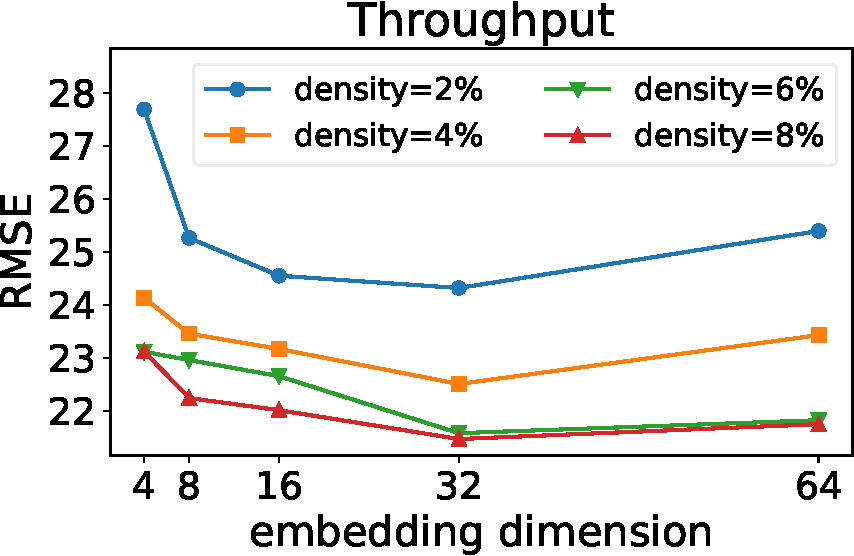
\includegraphics[width=0.85\textwidth]{figs/example.pdf}
    \caption{项目总体技术路线示意图}
    \label{fig:framework}
\end{figure}

\subsection{数据处理与数据集构建}
% 若使用公开数据集，应说明来源、引用、规模、字段、划分方式；
% 若自建数据集，应说明采集方式、标注规范、清洗流程和伦理/隐私处理。

如用到数据，说明数据来源、数据规模、字段含义、数据清洗、数据划分、数据增强、标注规范等。

\begin{table}[H]
    \centering
    \caption{数据集统计信息}
    \begin{tabular}{lcccc}
        \toprule
        数据集 & 样本数量 & 特征维度/字段数 & 训练/验证/测试划分 & 说明 \\
        \midrule
        数据集A & 10000 & 128 & 7:1:2 & 公开数据集/自建数据集 \\
        数据集B & 5000 & 64 & 8:1:1 & 用于泛化验证 \\
        \bottomrule
    \end{tabular}
    \label{tab:dataset}
\end{table}

数据预处理主要包括：缺失值处理、异常值剔除、数据标准化/归一化、样本划分、数据增强等。若涉及人工标注，需要说明标注规则、一致性检查方式和质量控制方法。

\subsection{核心算法/模型设计}
% 所有项目均建议保留本节。
% 研究型项目应详细写模型结构、关键公式、损失函数和训练过程。
% 系统开发型项目也应说明算法部分的输入输出、流程和实现方式。

所有项目均建议保留。研究型项目应详细说明模型结构、关键公式、训练目标和优化方法；系统开发型项目也应说明算法模块的输入、输出、流程和实现方式。

本项目设计的核心算法由\textbf{XXX模块、XXX模块和XXX模块}组成。其中，XXX模块用于\textbf{提取特征/建模关系/生成预测结果}；XXX模块用于\textbf{提升鲁棒性/融合多源信息/优化效率}。

\subsubsection{XXX模块}
% 描述模块功能、输入输出、关键公式、流程图或伪代码。

该模块的输入为 $X$，输出为 $H$。其主要作用是\textbf{XXX}，计算过程如下：
\begin{equation}
    H = \phi(WX+b),
    \label{eq:module}
\end{equation}
其中，$W$ 和 $b$ 为可学习参数，$\phi(\cdot)$ 表示非线性激活函数。

% 可附关键代码片段、更多实验结果、系统部署说明、用户手册等。
% 注意不要粘贴整个工程代码，只保留关键片段并说明作用。

\begin{lstlisting}[language=Python]
# 关键代码示例：根据实际项目替换
class ExampleModel:
    def __init__(self, config):
        self.config = config

    def forward(self, x):
        # 输入 x，输出预测结果 y_hat
        y_hat = x
        return y_hat
\end{lstlisting}

\subsubsection{目标函数与优化方法}
% 根据任务替换损失函数。

模型训练采用如下目标函数：
\begin{equation}
    \mathcal{L}=\mathcal{L}_{task}+\lambda\mathcal{L}_{reg},
    \label{eq:loss}
\end{equation}
其中，$\mathcal{L}_{task}$ 表示任务损失，$\mathcal{L}_{reg}$ 表示正则项，$\lambda$ 为权衡系数。

% 可附关键代码片段、更多实验结果、系统部署说明、用户手册等。
% 注意不要粘贴整个工程代码，只保留关键片段并说明作用。

\begin{lstlisting}[language=Python]
# 关键代码示例：根据实际项目替换
class ExampleModel:
    def __init__(self, config):
        self.config = config

    def forward(self, x):
        # 输入 x，输出预测结果 y_hat
        y_hat = x
        return y_hat
\end{lstlisting}

\subsection{系统开发设计与实现}
% 若项目不涉及系统开发，可删除本节。
% 系统型项目应先介绍算法部分，再介绍系统架构和功能实现。

（系统开发型项目保留）

系统开发型项目保留。建议包括：

需求分析；
系统架构；
功能模块设计；
数据库设计；
API接口设计；
部署与运行说明。

\subsubsection{需求分析}
% 从用户、功能、非功能需求三个角度说明。

系统面向\textbf{XXX用户}，主要支持\textbf{数据管理、模型推理、结果展示、用户交互、后台管理}等功能。系统需求包括：
\begin{itemize}
    \item 功能需求：支持\textbf{XXX功能、XXX功能、XXX功能}；
    \item 性能需求：页面响应时间、模型推理时间、并发访问能力等满足基本使用要求；
    \item 可用性需求：界面清晰、操作流程简单、结果展示直观；
    \item 安全性需求：对用户数据、上传文件或敏感信息进行必要保护。
\end{itemize}

\subsubsection{系统架构}
% 建议包含前端、后端、数据库、算法服务、部署环境等。

系统采用\textbf{前后端分离/前后端一体化}架构，主要由\textbf{前端展示层、业务逻辑层、算法服务层、数据存储层}组成。前端负责页面交互和结果可视化，后端负责业务逻辑、接口管理和权限控制，算法服务负责模型加载与推理，数据库用于存储用户、数据和结果信息。

\begin{figure}[H]
    \centering
    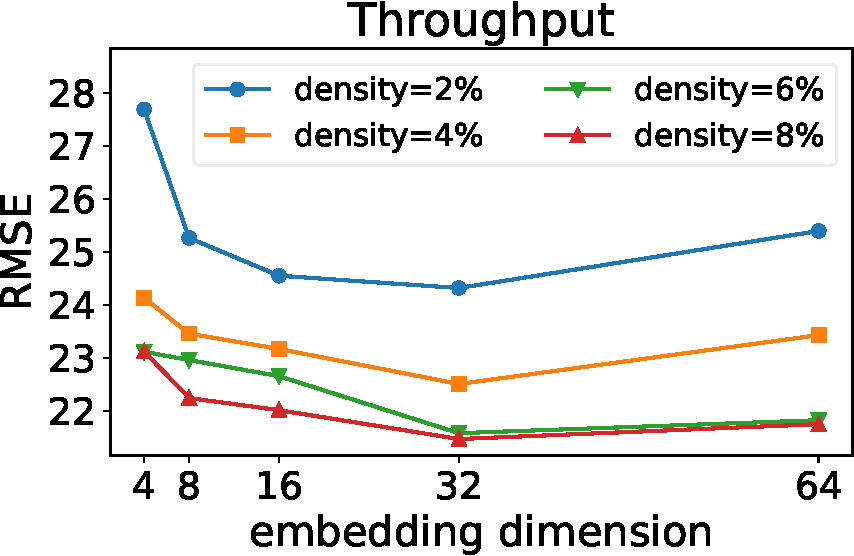
\includegraphics[width=0.85\textwidth]{figs/example.pdf}
    \caption{系统总体架构图}
    \label{fig:system_architecture}
\end{figure}

\subsubsection{功能模块设计与实现}

\begin{table}[H]
    \centering
    \caption{系统功能模块说明}
    \begin{tabular}{p{0.20\textwidth}p{0.35\textwidth}p{0.30\textwidth}}
        \toprule
        功能模块 & 主要功能 & 实现说明 \\
        \midrule
        数据管理模块 & 数据上传、查看、删除、预处理 & 使用XXX实现文件解析和数据清洗 \\
        模型推理模块 & 调用训练好的模型并返回预测结果 & 使用XXX加载模型，封装API接口 \\
        结果展示模块 & 展示指标、图表、可视化结果 & 使用XXX绘制图表或页面组件 \\
        后台管理模块 & 用户管理、日志管理、参数配置 & 使用XXX实现权限控制和数据维护 \\
        \bottomrule
    \end{tabular}
    \label{tab:function_modules}
\end{table}

% 可附关键代码片段、更多实验结果、系统部署说明、用户手册等。
% 注意不要粘贴整个工程代码，只保留关键片段并说明作用。

\begin{lstlisting}[language=Python]
# 关键代码示例：根据实际项目替换
class ExampleModel:
    def __init__(self, config):
        self.config = config

    def forward(self, x):
        # 输入 x，输出预测结果 y_hat
        y_hat = x
        return y_hat
\end{lstlisting}

\subsubsection{数据库/API/部署设计}
% 根据项目实际选择保留。

若使用数据库，需要说明核心数据表及字段设计；若提供API接口，需要说明接口路径、请求参数和返回结果；若完成部署，需要说明部署环境、运行方式和访问地址。

\begin{table}[H]
    \centering
    \caption{核心接口设计示例}
    \begin{tabular}{llll}
        \toprule
        接口名称 & 请求方式 & 接口路径 & 功能说明 \\
        \midrule
        数据上传 & POST & /api/upload & 上传实验数据 \\
        模型预测 & POST & /api/predict & 调用模型生成预测结果 \\
        结果查询 & GET & /api/results & 查询历史实验结果 \\
        \bottomrule
    \end{tabular}
    \label{tab:api}
\end{table}




\section{实验设置与评价方法}
% 研究型项目必须写充分；系统开发型项目若包含算法实验也应保留。

\textbf{（研究型项目重点保留）}

\subsection{实验环境}
% 说明硬件、软件、语言、框架、CUDA版本、主要依赖库等。

\begin{table}[H]
    \centering
    \caption{实验环境配置}
    \begin{tabular}{ll}
        \toprule
        项目 & 配置 \\
        \midrule
        操作系统 & Ubuntu 22.04 / Windows 11 \\
        CPU & XXX \\
        GPU & XXX \\
        编程语言 & Python 3.X \\
        深度学习框架 & PyTorch X.X / TensorFlow X.X \\
        其他依赖 & NumPy, Pandas, Scikit-learn等 \\
        \bottomrule
    \end{tabular}
    \label{tab:env}
\end{table}

\subsection{基准方法}
% 研究型项目应选择若干有代表性的传统方法、经典模型和较新方法作为基线。
% 系统型项目也可将不同算法版本作为对比方法。

本文选择以下方法作为对比基准：
\begin{itemize}
    \item 基线方法1：XXX，代表传统机器学习方法；
    \item 基线方法2：XXX，代表经典深度学习方法；
    \item 基线方法3：XXX，代表近年来相关研究中的先进方法；
    \item 本项目方法：XXX，即本文设计的最终方法。
\end{itemize}

\subsection{评价指标}
% 说明指标名称、含义、越大越好/越小越好，并给出必要公式。

本项目采用\textbf{准确率、召回率、F1值、MAE、RMSE、NDCG、运行时间}等指标评价模型性能。以准确率为例，其定义如下：
\begin{equation}
    \mathrm{ACC}=\frac{N_{correct}}{N_{total}},
    \label{eq:acc}
\end{equation}
其中，$N_{correct}$ 表示预测正确的样本数量，$N_{total}$ 表示样本总数量。

\subsection{参数设置与复现说明}
% 说明训练轮数、学习率、batch size、优化器、早停策略、随机种子等。

模型训练采用XXX优化器，学习率为XXX，批大小为XXX，训练轮数为XXX，早停轮数为XXX。为保证实验可复现，本文固定随机种子为XXX，并在相同数据划分和实验环境下进行对比实验。

\section{项目成果展示与分析}
% 本节是结题报告的核心。根据项目类型选择保留“研究型成果”或“系统开发型成果”，也可以两者都保留。

\subsection{研究型成果展示与分析（研究型项目保留）}
% 研究型项目应尽量形成类似学术论文的实验结构。

\subsubsection{主要实验结果}
% 与基线方法进行定量对比。注意说明最优、次优、提升幅度。

\begin{table}[H]
    \centering
    \caption{不同方法在主要数据集上的性能比较}
    \begin{tabular}{lccc}
        \toprule
        方法 & 指标1 $\uparrow$ & 指标2 $\uparrow$ & 指标3 $\downarrow$ \\
        \midrule
        Baseline 1 & 0.812 & 0.735 & 0.245 \\
        Baseline 2 & 0.846 & 0.762 & 0.218 \\
        本项目方法 & \textbf{0.891} & \textbf{0.806} & \textbf{0.176} \\
        \bottomrule
    \end{tabular}
    \label{tab:main_results}
\end{table}

从表\ref{tab:main_results}可以看出，本项目方法在\textbf{XXX指标}上优于对比方法，说明所设计的\textbf{XXX模块/策略}能够有效提升模型性能。与最强基线相比，本项目方法在\textbf{XXX指标}上提升了\textbf{X\%}。

\subsubsection{模型比较与结果分析}
% 分析不同方法为什么好/不好，不要只重复表格数字。

对比实验表明，传统方法在\textbf{XXX方面}表现有限，主要原因是其难以捕捉\textbf{复杂非线性关系/长程依赖/多模态特征}；深度学习方法能够获得更好的性能，但在\textbf{鲁棒性/效率/可解释性}方面仍有不足。本项目方法通过\textbf{XXX设计}缓解了上述问题。

\subsubsection{消融实验}
% 用于证明各个模块是否真的有效。

\begin{table}[H]
    \centering
    \caption{消融实验结果}
    \begin{tabular}{lccc}
        \toprule
        模型变体 & 指标1 $\uparrow$ & 指标2 $\uparrow$ & 指标3 $\downarrow$ \\
        \midrule
        完整模型 & \textbf{0.891} & \textbf{0.806} & \textbf{0.176} \\
        去除模块A & 0.865 & 0.781 & 0.201 \\
        去除模块B & 0.872 & 0.790 & 0.193 \\
        替换模块C & 0.854 & 0.773 & 0.210 \\
        \bottomrule
    \end{tabular}
    \label{tab:ablation}
\end{table}

消融实验结果说明，模块A、模块B和模块C均对最终性能具有积极贡献。其中，去除模块A后性能下降最明显，表明该模块是提升模型效果的关键组成部分。

\subsubsection{超参数影响分析}
% 选择1--3个关键超参数进行分析，不宜过多。

\begin{figure}[H]
    \centering
    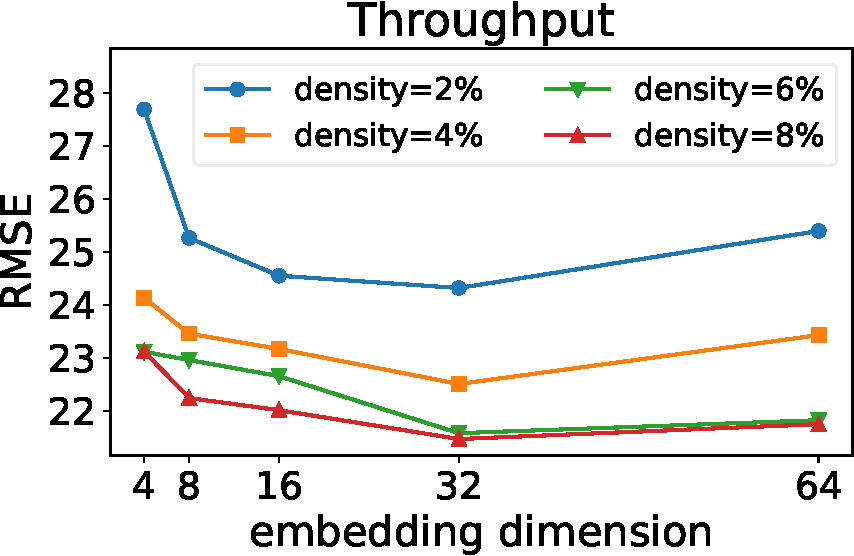
\includegraphics[width=0.70\textwidth]{figs/example.pdf}
    \caption{关键超参数对模型性能的影响}
    \label{fig:hyper}
\end{figure}

图\ref{fig:hyper}展示了关键超参数对模型性能的影响。当参数取值为XXX时，模型性能达到最优；当参数继续增大时，模型可能出现过拟合或计算开销增加的问题。

\subsubsection{效率分析}
% 可分析训练时间、推理时间、参数量、内存占用等。

\begin{table}[H]
    \centering
    \caption{效率对比结果}
    \begin{tabular}{lccc}
        \toprule
        方法 & 参数量 & 训练时间 / s & 推理时间 / ms \\
        \midrule
        Baseline 1 & 1.2M & 120 & 8.5 \\
        Baseline 2 & 2.5M & 180 & 10.2 \\
        本项目方法 & 1.8M & 150 & 7.9 \\
        \bottomrule
    \end{tabular}
    \label{tab:efficiency}
\end{table}

\subsubsection{案例分析与可视化分析}
% 可展示典型成功案例、失败案例、注意力图、特征分布、混淆矩阵等。

通过对典型样本进行分析可以发现，本项目方法在\textbf{XXX场景}下能够得到更准确的结果。但在\textbf{XXX复杂场景}下仍存在错误，说明后续还需要进一步提升模型对\textbf{噪声、长尾样本或分布变化}的适应能力。



\subsection{系统开发型成果展示与分析}
% 系统型项目需要说明“算法有效 + 系统可用”。

\textbf{（系统开发型项目保留）}

\subsubsection{系统功能完成情况}

\begin{table}[H]
    \centering
    \caption{系统功能完成情况}
    \begin{tabular}{p{0.22\textwidth}p{0.40\textwidth}p{0.18\textwidth}p{0.12\textwidth}}
        \toprule
        功能模块 & 功能说明 & 实现状态 & 完成度 \\
        \midrule
        用户登录模块 & 支持用户注册、登录、身份校验 & 已完成 & 100\% \\
        数据管理模块 & 支持数据上传、预览、删除与清洗 & 已完成 & 95\% \\
        算法推理模块 & 支持调用模型并返回预测结果 & 已完成 & 90\% \\
        可视化展示模块 & 支持图表展示、结果下载与案例分析 & 已完成 & 90\% \\
        \bottomrule
    \end{tabular}
    \label{tab:system_completion}
\end{table}

\subsubsection{系统界面与运行效果展示}
% 建议放置系统首页、核心功能页面、结果展示页面、后台管理页面等截图。

\begin{figure}[H]
    \centering
    \subfigure[系统首页]{
        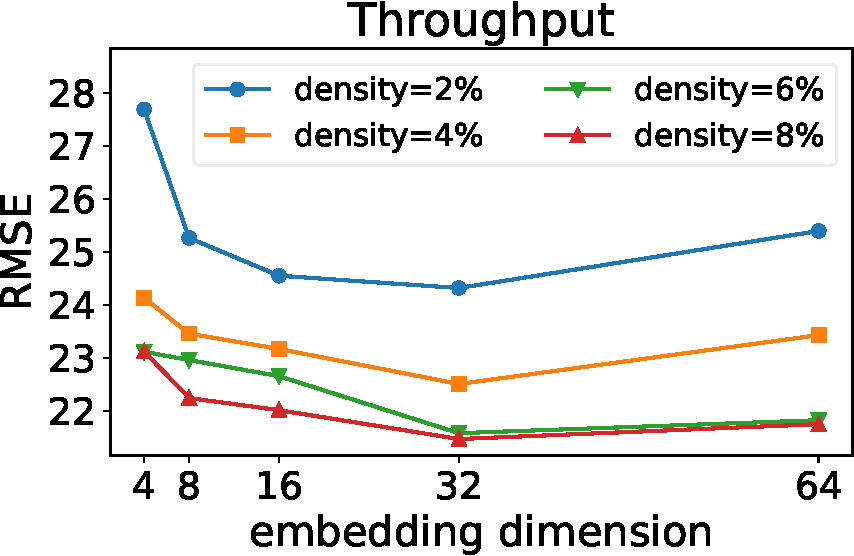
\includegraphics[width=0.45\linewidth]{figs/example.pdf}
    }\hfill
    \subfigure[结果展示页面]{
        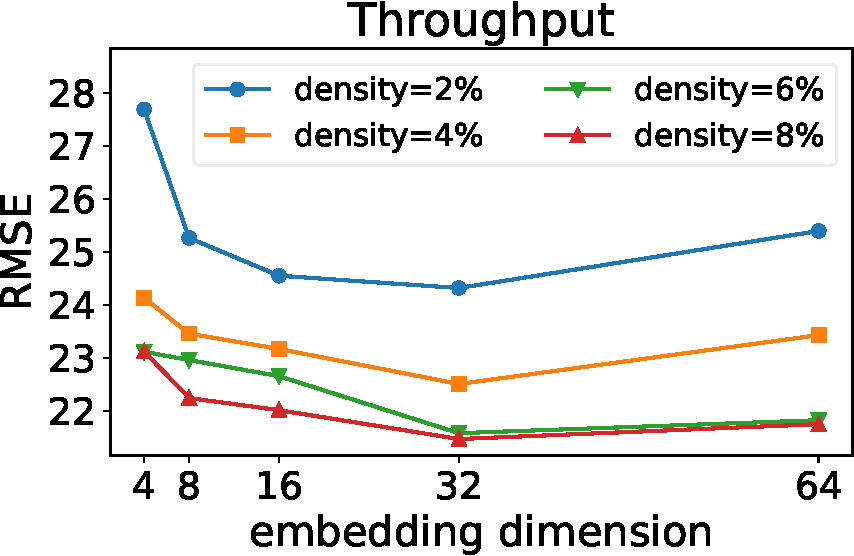
\includegraphics[width=0.45\linewidth]{figs/example.pdf}
    }
    \caption{系统界面展示示例}
    \label{fig:system_demo}
\end{figure}

\subsubsection{系统测试与性能分析}
% 可包含功能测试、接口测试、响应时间测试、异常输入测试等。

\begin{table}[H]
    \centering
    \caption{系统测试结果}
    \begin{tabular}{llll}
        \toprule
        测试项目 & 测试内容 & 测试结果 & 是否通过 \\
        \midrule
        功能测试 & 数据上传、模型预测、结果展示 & 运行正常 & 通过 \\
        接口测试 & API请求与返回格式检查 & 返回正确 & 通过 \\
        异常测试 & 空文件、错误格式、非法输入 & 能够提示错误 & 通过 \\
        性能测试 & 单次预测响应时间 & 平均XXX ms & 通过 \\
        \bottomrule
    \end{tabular}
    \label{tab:system_test}
\end{table}

\subsubsection{算法模块在系统中的应用效果}
% 系统项目不能只展示页面，还应说明算法模块是否有效。

在系统运行过程中，算法模块主要用于\textbf{XXX功能}。通过对XXX组测试样例进行验证，系统能够在平均XXX秒内返回结果，预测准确率/推荐效果/检测效果达到XXX，说明算法模块能够满足原型系统的基本应用需求。

\subsection{其他成果}
% 根据实际情况填写，如论文、竞赛、软著、专利、开源代码、数据集、演示视频等。

本项目形成的其他成果包括：
\begin{itemize}
    \item 代码仓库：XXX；
    \item 数据集或数据处理脚本：XXX；
    \item 原型系统或演示视频：XXX；
    \item 论文/报告/专利/软著/竞赛成果：XXX；
    \item 项目文档：需求文档、设计文档、测试文档、用户手册等。
\end{itemize}

\section{创新点与特色}
% 不宜写得过大，应围绕本项目真实完成的工作总结。
% 建议从问题、方法、数据、系统、应用五个角度选择2--4点。

本项目的创新点和特色主要体现在以下方面：
\begin{itemize}
    \item 创新点1：针对\textbf{XXX问题}，提出了\textbf{XXX建模思路/算法模块}；
    \item 创新点2：构建了\textbf{XXX数据集/实验流程/评价方案}，为项目验证提供了数据基础；
    \item 创新点3：将\textbf{XXX算法}集成到\textbf{XXX系统}中，实现了从模型设计到系统应用的完整流程；
    \item 创新点4：通过\textbf{消融实验、超参数分析、案例分析、系统测试}等方式，对项目成果进行了较充分验证。
\end{itemize}



\section{存在问题、不足与改进方向}
% 结题报告应客观说明不足，不宜只写优点。

尽管本项目完成了预定目标，但仍存在以下不足：
\begin{itemize}
    \item 数据方面：数据规模仍然有限，样本分布可能不够均衡，数据质量有待进一步提高；
    \item 方法方面：模型在复杂场景或长尾样本上的表现仍有提升空间；
    \item 实验方面：目前对比方法、消融设置或多数据集验证仍可进一步丰富；
    \item 系统方面：原型系统在并发访问、异常处理、权限控制和部署稳定性方面仍需完善。
\end{itemize}

后续可从以下方向继续改进：扩大数据规模、引入更强的模型结构、完善系统功能、提升系统部署稳定性、增加用户测试和实际应用验证等。

\section{总结}
% 用一段总结项目完成情况、主要成果、能力提升和后续价值。

本项目围绕\textbf{XXX问题}，完成了从\textbf{背景调研、问题定义、方案设计、算法实现、实验验证到系统展示}的完整实践过程。实验结果/系统测试表明，项目所提出的方法/实现的系统能够较好地完成预期任务。通过本项目，团队成员在\textbf{文献调研、算法建模、程序实现、实验分析、系统开发、项目协作和报告撰写}等方面得到了较为系统的训练。

\section{心得体会}
% 可由每位成员分别撰写，也可统一撰写。
% 建议包括：遇到的问题、解决过程、能力提升、对课程/科研/工程实践的认识。

通过本次创新实验，对\textbf{XXX领域}有了更加深入的理解，也掌握了\textbf{数据处理、模型设计、实验评估、系统实现}等关键实践技能。在项目推进过程中，遇到了\textbf{XXX困难}，并通过\textbf{查阅文献、调试代码、调整方案、团队协作}等方式逐步解决。后续将继续围绕\textbf{XXX方向}完善项目成果。

\bibliography{ref}
% 参考文献主要包含实验过程中涉及到的文献、数据集来源、开源代码、工具文档等。


\end{document}
